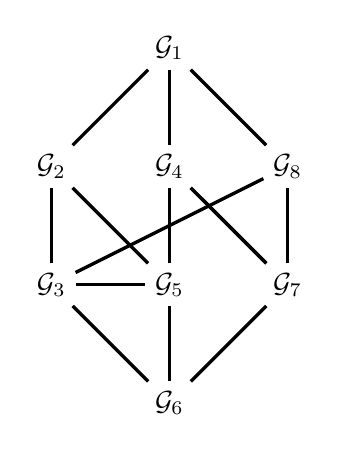
\begin{tikzpicture}[scale = 0.5]
\node (A) at (0,0) {$\mathcal{G}_{1}$};

\node (C) at (-3,-3) {$\mathcal{G}_{2}$};
\node (D) at (0,-3) {$\mathcal{G}_{4}$};
\node (B) at (3,-3) {$\mathcal{G}_{8}$};

\node (E) at (3,-6) {$\mathcal{G}_{7}$};
\node (F) at (-3,-6) {$\mathcal{G}_{3}$};
\node (G) at (0,-6) {$\mathcal{G}_{5}$};

\node (H) at (0,-9) {$\mathcal{G}_{6}$};


\draw[-, very thick] (D) to (A);
\draw[-, very thick] (C) to (A);
\draw[-, very thick] (B) to (A);

\draw[-, very thick] (E) to (D);
\draw[-, very thick] (F) to (C);
\draw[-, very thick] (G) to (D);
\draw[-, very thick] (G) to (C);
\draw[-, very thick] (E) to (D);
\draw[-, very thick] (F) to (B);
\draw[-, very thick] (E) to (B);

\draw[-, very thick] (H) to (G);
\draw[-, very thick] (H) to (F);
\draw[-, very thick] (H) to (E);
\draw[-, very thick] (F) to (G);

\end{tikzpicture}